% Mini research note for the canonical single-mode Raman-suppression baseline.
\documentclass[11pt]{article}
% Shared preamble for the research-note series.
% Create note-specific content in the per-note directory; keep common macros here.
\usepackage[margin=1in]{geometry}
\usepackage[T1]{fontenc}
\usepackage[utf8]{inputenc}
\usepackage{amsmath,amssymb}
\usepackage{booktabs,longtable,array}
\usepackage{graphicx}
\usepackage{float}
\usepackage{enumitem}
\usepackage{xcolor}
\usepackage{hyperref}
\usepackage{caption}
\usepackage{titlesec}
\hypersetup{colorlinks=true, linkcolor=blue!60!black, urlcolor=blue!60!black, citecolor=blue!60!black}
\setlist[itemize]{leftmargin=1.25em, itemsep=0.2em, topsep=0.3em}
\setlist[enumerate]{leftmargin=1.4em, itemsep=0.2em, topsep=0.3em}
\setlength{\parindent}{0pt}
\setlength{\parskip}{0.6em}
\newcommand{\statusbox}[2]{%
  \noindent\fcolorbox{black}{gray!10}{%
    \parbox{\dimexpr\linewidth-2\fboxsep-2\fboxrule\relax}{%
      \textbf{Status:} #1\\#2
    }%
  }
}

% Shared notation helpers for the research-note series.
\newcommand{\Jlin}{J}
\newcommand{\Jphys}{J_{\mathrm{phys}}}
\newcommand{\Jsurf}{J_{\mathrm{surf}}}
\newcommand{\JdB}{J_{\mathrm{dB}}}
\newcommand{\phiopt}{\phi_{\mathrm{opt}}}
\newcommand{\sigmathreedb}{\sigma_{3\mathrm{dB}}}
\newcommand{\Nt}{N_t}
\newcommand{\Nphi}{N_{\phi}}
\newcommand{\Lfiber}{L}
\newcommand{\Pcont}{P}
\newcommand{\band}{\mathcal{B}_{\mathrm{Raman}}}
\newcommand{\todoitem}[1]{\textcolor{red!70!black}{\textbf{TODO:} #1}}


\title{Baseline Raman Suppression and Core Optimization Surface}
\author{Fiber Raman Suppression Project}
\date{Evidence snapshot: 2026-04-26}

\begin{document}
\maketitle

\begin{abstract}
This note is the front door to the project. It explains the baseline
single-mode, phase-only Raman-suppression experiment: choose an input spectral
phase, propagate the pulse through a nonlinear fiber model, and minimize the
fraction of output energy that lands in the Raman-shifted band. The canonical
SMF-28 run shown here improves the Raman-band objective from
\(-1.11\,\mathrm{dB}\) without shaping to \(-44.79\,\mathrm{dB}\) after
optimization, while passing the numerical trust checks. The baseline is not
the deepest path in the repo. Its purpose is to define the physics, objective,
diagnostics, and vocabulary that all later research directions modify.
\end{abstract}

\section*{Claim Status}
\statusbox{established reference workflow}{The single-mode phase-only workflow
is stable enough to serve as the common baseline for the research-note series.
The strongest claim is methodological: the project has a coherent objective,
adjoint-gradient optimizer, no-optimization control, standard image bundle, and
trust-report gate. Deeper optimization strategies are covered in separate
notes.}

\section{Question and Thesis}

The baseline question is whether phase-only input shaping can suppress
Raman-band energy in a clean, reproducible single-mode fiber experiment.

The answer is yes. The maintained baseline changes only the spectral phase
\(\phi(\omega)\), keeps the input amplitude fixed, propagates through a
single-mode nonlinear fiber model, and minimizes the output Raman-band energy
fraction. That gives a deliberately narrow reference problem:
\[
    \text{phase-only control}
    \quad\Longrightarrow\quad
    \text{lower Raman-band output fraction}.
\]

This matters because every later path changes one piece of this setup.
Reduced-basis work changes the allowed phase shapes. Sharpness work changes
the objective so local robustness matters. Trust-region work changes the
optimizer. Long-reach and multimode work change the physical model. This note
defines the common object those paths start from.

\subsection*{Intuition Check}

Think of the pulse as many colors traveling together. Raman scattering moves
energy toward longer wavelengths. The phase mask tries to rearrange the timing
of those colors before the fiber so the nonlinear evolution sends less energy
into the unwanted Raman-shifted region.

\section{Physical Problem}

The canonical benchmark in this note is
\[
    \text{SMF-28},\qquad
    L=2\,\mathrm{m},\qquad
    P=0.2\,\mathrm{W},\qquad
    \lambda_0=1550\,\mathrm{nm}.
\]
The maintained run uses \(\Nt=8192\), a \(27\,\mathrm{ps}\) time window, and a
\(185\,\mathrm{fs}\) input pulse. The fiber propagation follows the generalized
nonlinear Schr\"odinger equation, with dispersion, Kerr nonlinearity, and Raman
response as in standard nonlinear-fiber optics \cite{agrawal2019,dudley2006}.
The numerical propagation style follows interaction-picture / split-step ideas
used for supercontinuum and nonlinear pulse simulations \cite{hult2007}.

\begin{figure}[H]
\centering
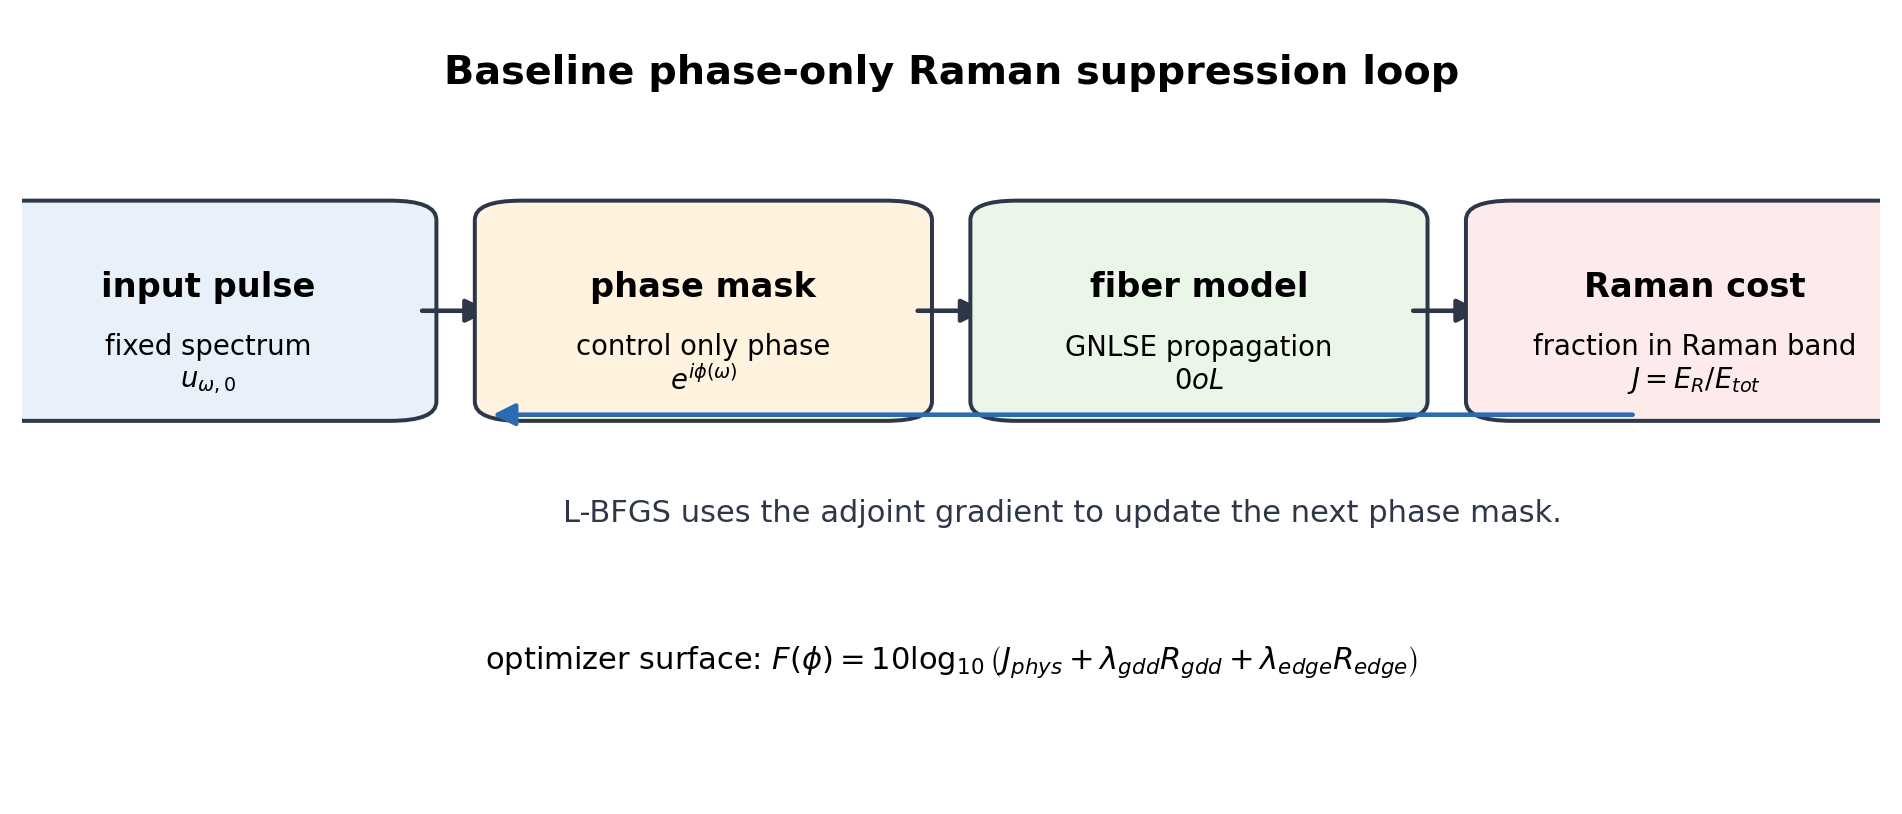
\includegraphics[width=0.95\linewidth]{figures/baseline_workflow_clean.png}
\caption{Baseline phase-only optimization loop. The optimizer proposes a
spectral phase, the nonlinear fiber solver propagates the shaped pulse, the
Raman-band output fraction is measured, and the adjoint gradient tells L-BFGS
how to update the phase.}
\end{figure}

The shaped input spectrum is
\[
    u_\omega(0;\phi)=u_{\omega,0}\exp(i\phi(\omega)).
\]
Only phase is changed. The spectral amplitude is not intentionally reduced, so
the optimizer cannot win by throwing away input energy. This is why the result
is physically meaningful as a phase-shaping result rather than an attenuation
trick.

\subsection*{Intuition Check}

Amplitude shaping can suppress unwanted output partly by deleting input power.
Phase shaping is a stricter test: the same colors are still present, but their
relative timing is changed.

\section{The Objective}

At the fiber output, define the Raman-band energy and total output energy:
\[
    E_{\band}(\phi)
    =
    \sum_{\omega_k\in\band}|u_{\omega_k}(L;\phi)|^2\,\Delta\omega,
    \qquad
    E_{\mathrm{tot}}(\phi)
    =
    \sum_k |u_{\omega_k}(L;\phi)|^2\,\Delta\omega.
\]
The physics cost is the fraction
\[
    \Jphys(\phi)=\frac{E_{\band}(\phi)}{E_{\mathrm{tot}}(\phi)}.
\]
Lower is better. The reported value is usually
\[
    \JdB(\phi)=10\log_{10}\Jphys(\phi).
\]
For example, \(-40\,\mathrm{dB}\) means roughly \(10^{-4}\) of the output
energy lies in the Raman band.

The maintained optimizer uses a regularized linear surface before applying the
dB transform:
\[
    \Jsurf(\phi)
    =
    \Jphys(\phi)
    +\lambda_{\mathrm{gdd}}R_{\mathrm{gdd}}(\phi)
    +\lambda_{\mathrm{edge}}R_{\mathrm{edge}}(\phi),
\]
with the canonical settings
\[
    \lambda_{\mathrm{gdd}}=10^{-4},
    \qquad
    \lambda_{\mathrm{edge}}=1.
\]
The scalar passed to L-BFGS is
\[
    F(\phi)=10\log_{10}\Jsurf(\phi).
\]

\begin{figure}[H]
\centering
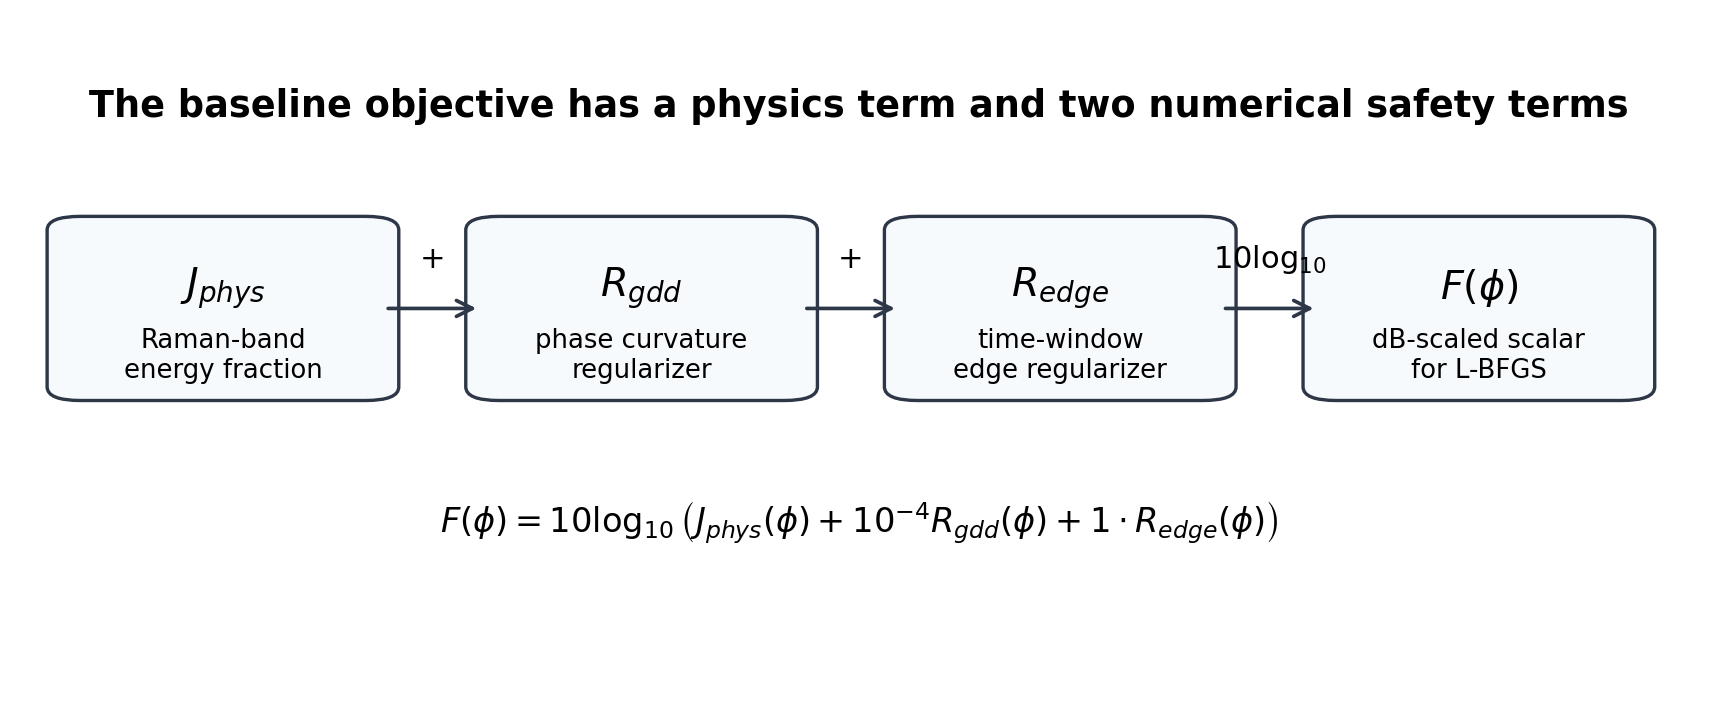
\includegraphics[width=0.90\linewidth]{figures/baseline_cost_anatomy.png}
\caption{Baseline objective anatomy. The physics term measures Raman-band
energy fraction. The two regularizers are numerical safety terms. The dB
transform is applied after the full linear surface is assembled.}
\end{figure}

The gradient must match the same scalar surface:
\[
    \nabla_\phi F
    =
    \frac{10}{\ln 10}
    \frac{1}{\Jsurf(\phi)}
    \nabla_\phi \Jsurf.
\]
This chain-rule scaling is important because the Raman fraction can become
very small. The dB surface keeps the optimizer from losing useful gradient
scale in deep-suppression regimes.

\subsection*{Intuition Check}

The regularizers are not the main scientific result. They are guardrails. The
main target is still ``make the Raman-band fraction small.'' The guardrails
discourage numerically suspicious phase curvature and pulses that touch the
edge of the simulation time window.

\section{Adjoint Gradient and L-BFGS}

The high-dimensional part of the problem is the phase vector. With
\(\Nt=8192\), finite differences would be too expensive: one would need
thousands of extra forward propagations to estimate a gradient.

The project instead uses an adjoint method. A forward solve gives the output
field. A backward adjoint solve starts from the derivative of the output cost
and propagates sensitivity back to the input. The phase-gradient form is
\[
    \frac{d F}{d \phi(\omega)}
    \propto
    \operatorname{Re}\!\left[
    \lambda_0(\omega)^\ast\, i\,u_\omega(0;\phi)
    \right],
\]
with the proportionality including the dB scaling and regularizer gradients.
L-BFGS then uses this gradient to update the phase without forming a full
Hessian \cite{liu1989,nocedal2006}.

\subsection*{Intuition Check}

The adjoint is a shortcut for asking a very large ``what if?'' question. It
answers, all at once, which phase pixels should move up or down to reduce the
Raman-band output.

\section{Implementation Surface}

\begin{center}
\small
\begin{tabular}{>{\raggedright\arraybackslash}p{0.30\linewidth}
                >{\raggedright\arraybackslash}p{0.60\linewidth}}
\toprule
\textbf{Component} & \textbf{Role in the baseline workflow} \\
\midrule
Canonical driver & Supported public entry point for the canonical single-mode
optimization run. \\
Workflow wrapper & Dispatches approved run identifiers and output directories. \\
Optimization library & Defines the single-mode cost, adjoint-gradient wrapper,
L-BFGS call, result payload, and trust report. \\
Problem setup & Builds the pulse, fiber, simulation grid, Raman-band mask, and
shared simulation containers. \\
Standard-image helper & Saves the phase profile, phase diagnostic, optimized
evolution heat map, and unshaped evolution heat map. \\
Cost-convention document & Defines the rule that regularizers are added before
any optional dB transform. \\
\bottomrule
\end{tabular}
\end{center}

The code names are intentionally kept out of the main story. For reproduction,
the relevant paths are listed in the README next to this note.

\section{Experimental Method}

The maintained baseline experiment has five steps:
\begin{enumerate}
    \item build the SMF-28 pulse, fiber, grid, and Raman-band mask;
    \item evaluate the no-shaping control \(\phi\equiv0\);
    \item run L-BFGS on the regularized dB objective;
    \item save the standard image set for the shaped result and the unshaped
    control;
    \item check determinism, boundary energy, photon conservation, gradient
    validation, and objective-surface metadata.
\end{enumerate}

\begin{figure}[H]
\centering
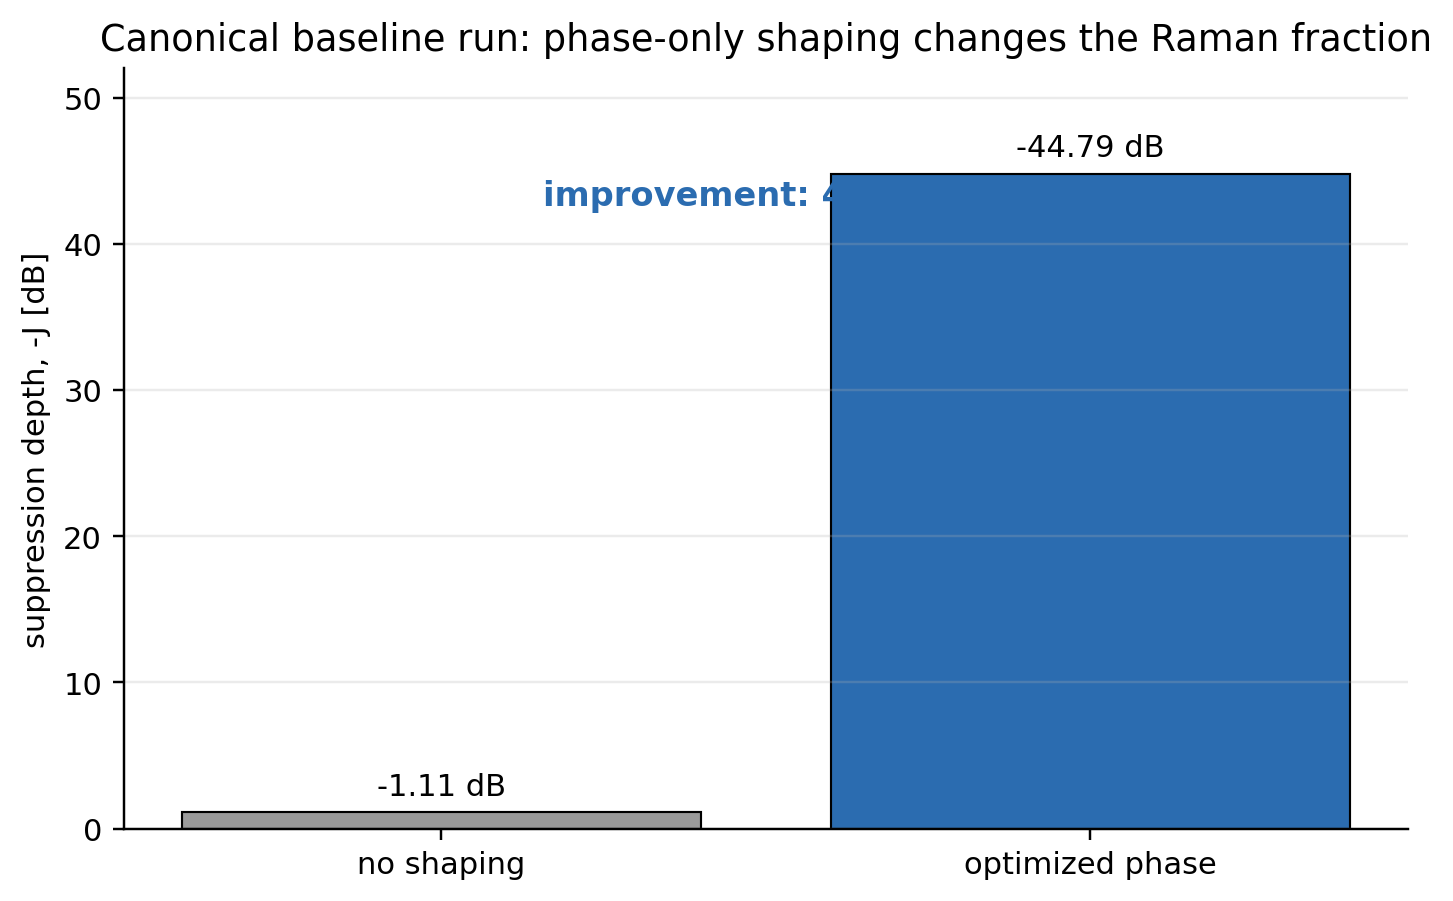
\includegraphics[width=0.72\linewidth]{figures/baseline_before_after_summary.png}
\caption{Canonical baseline scalar result. The no-shaping Raman-band fraction
is \(-1.11\,\mathrm{dB}\); the optimized phase reaches
\(-44.79\,\mathrm{dB}\), a \(43.68\,\mathrm{dB}\) improvement.}
\end{figure}

\begin{center}
\small
\begin{tabular}{>{\raggedright\arraybackslash}p{0.44\linewidth}
                >{\raggedright\arraybackslash}p{0.42\linewidth}}
\toprule
\textbf{Quantity} & \textbf{Canonical run value} \\
\midrule
Fiber and operating point & SMF-28, \(L=2\,\mathrm{m}\), \(P=0.2\,\mathrm{W}\) \\
Grid & \(\Nt=8192\), \(27\,\mathrm{ps}\) time window \\
Input pulse & \(185\,\mathrm{fs}\), centered at \(1550\,\mathrm{nm}\) \\
Initial objective & \(-1.11\,\mathrm{dB}\) \\
Final objective & \(-44.79\,\mathrm{dB}\) \\
Iterations & 47 \\
Converged flag & true \\
\bottomrule
\end{tabular}
\end{center}

\begin{figure}[H]
\centering
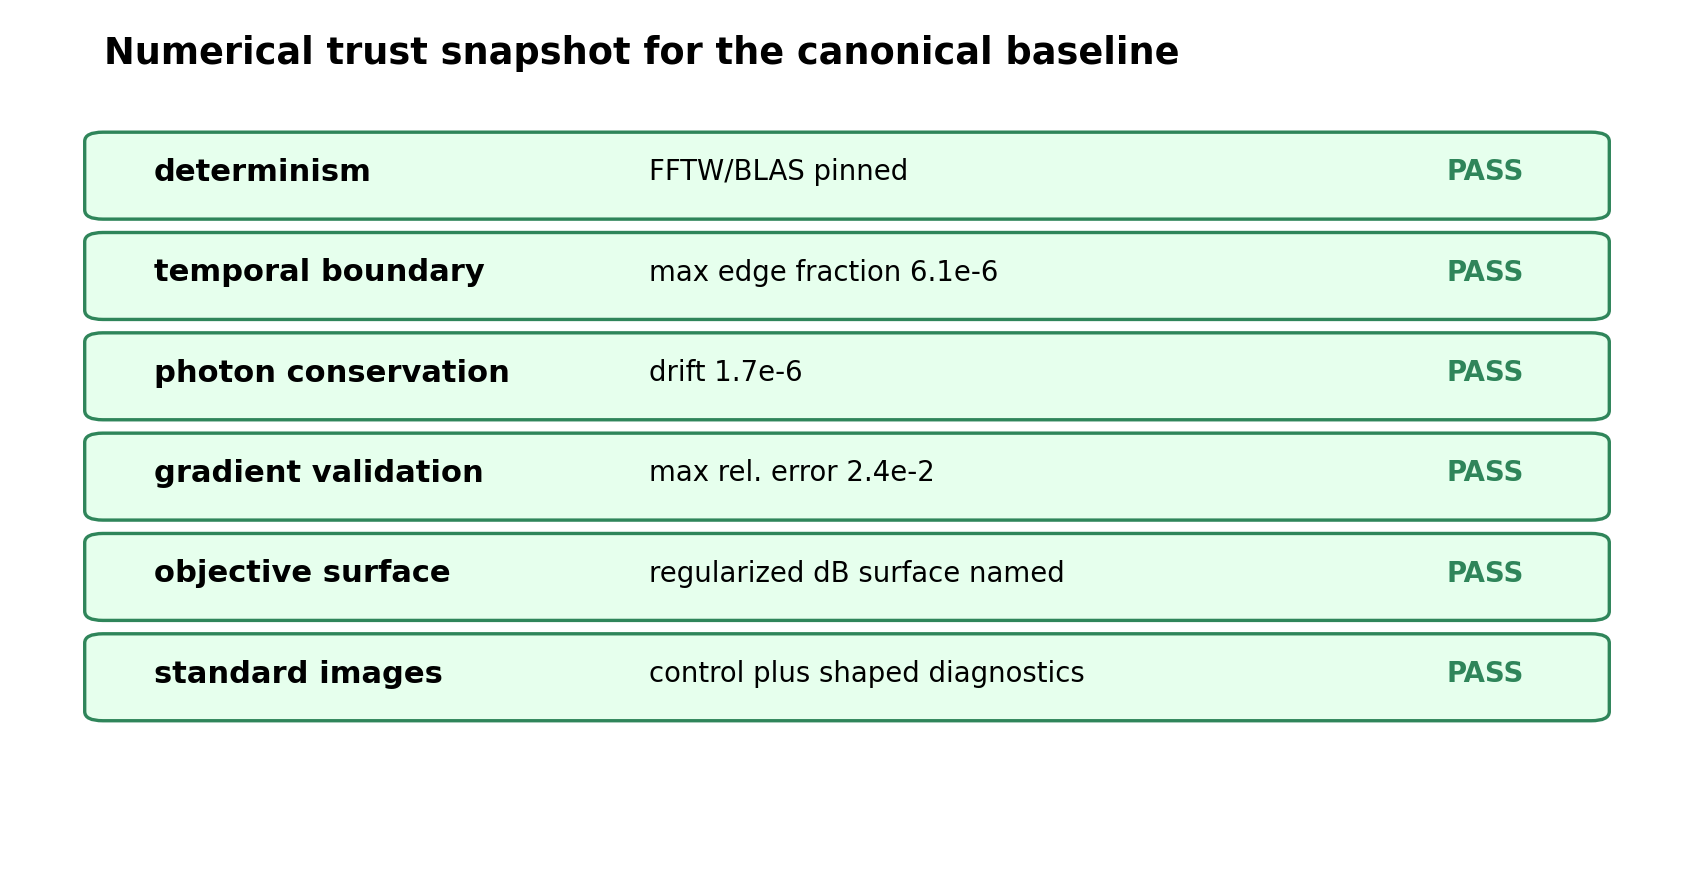
\includegraphics[width=0.86\linewidth]{figures/baseline_trust_snapshot.png}
\caption{Numerical trust snapshot for the canonical run. The run passes the
determinism, boundary, photon-conservation, gradient-validation,
objective-surface, and standard-image gates.}
\end{figure}

\subsection*{Intuition Check}

This is why the baseline is useful. It is not just a low number. It is a low
number with a control group, a named objective, a gradient check, and pictures
showing what phase was applied and what spectral evolution followed.

\clearpage
\section{Representative Result Pages}

The pages below pair each phase diagnostic with the corresponding spectral
evolution heat map. This is the standard format for the rest of the note
series.

\begin{figure}[p]
\centering
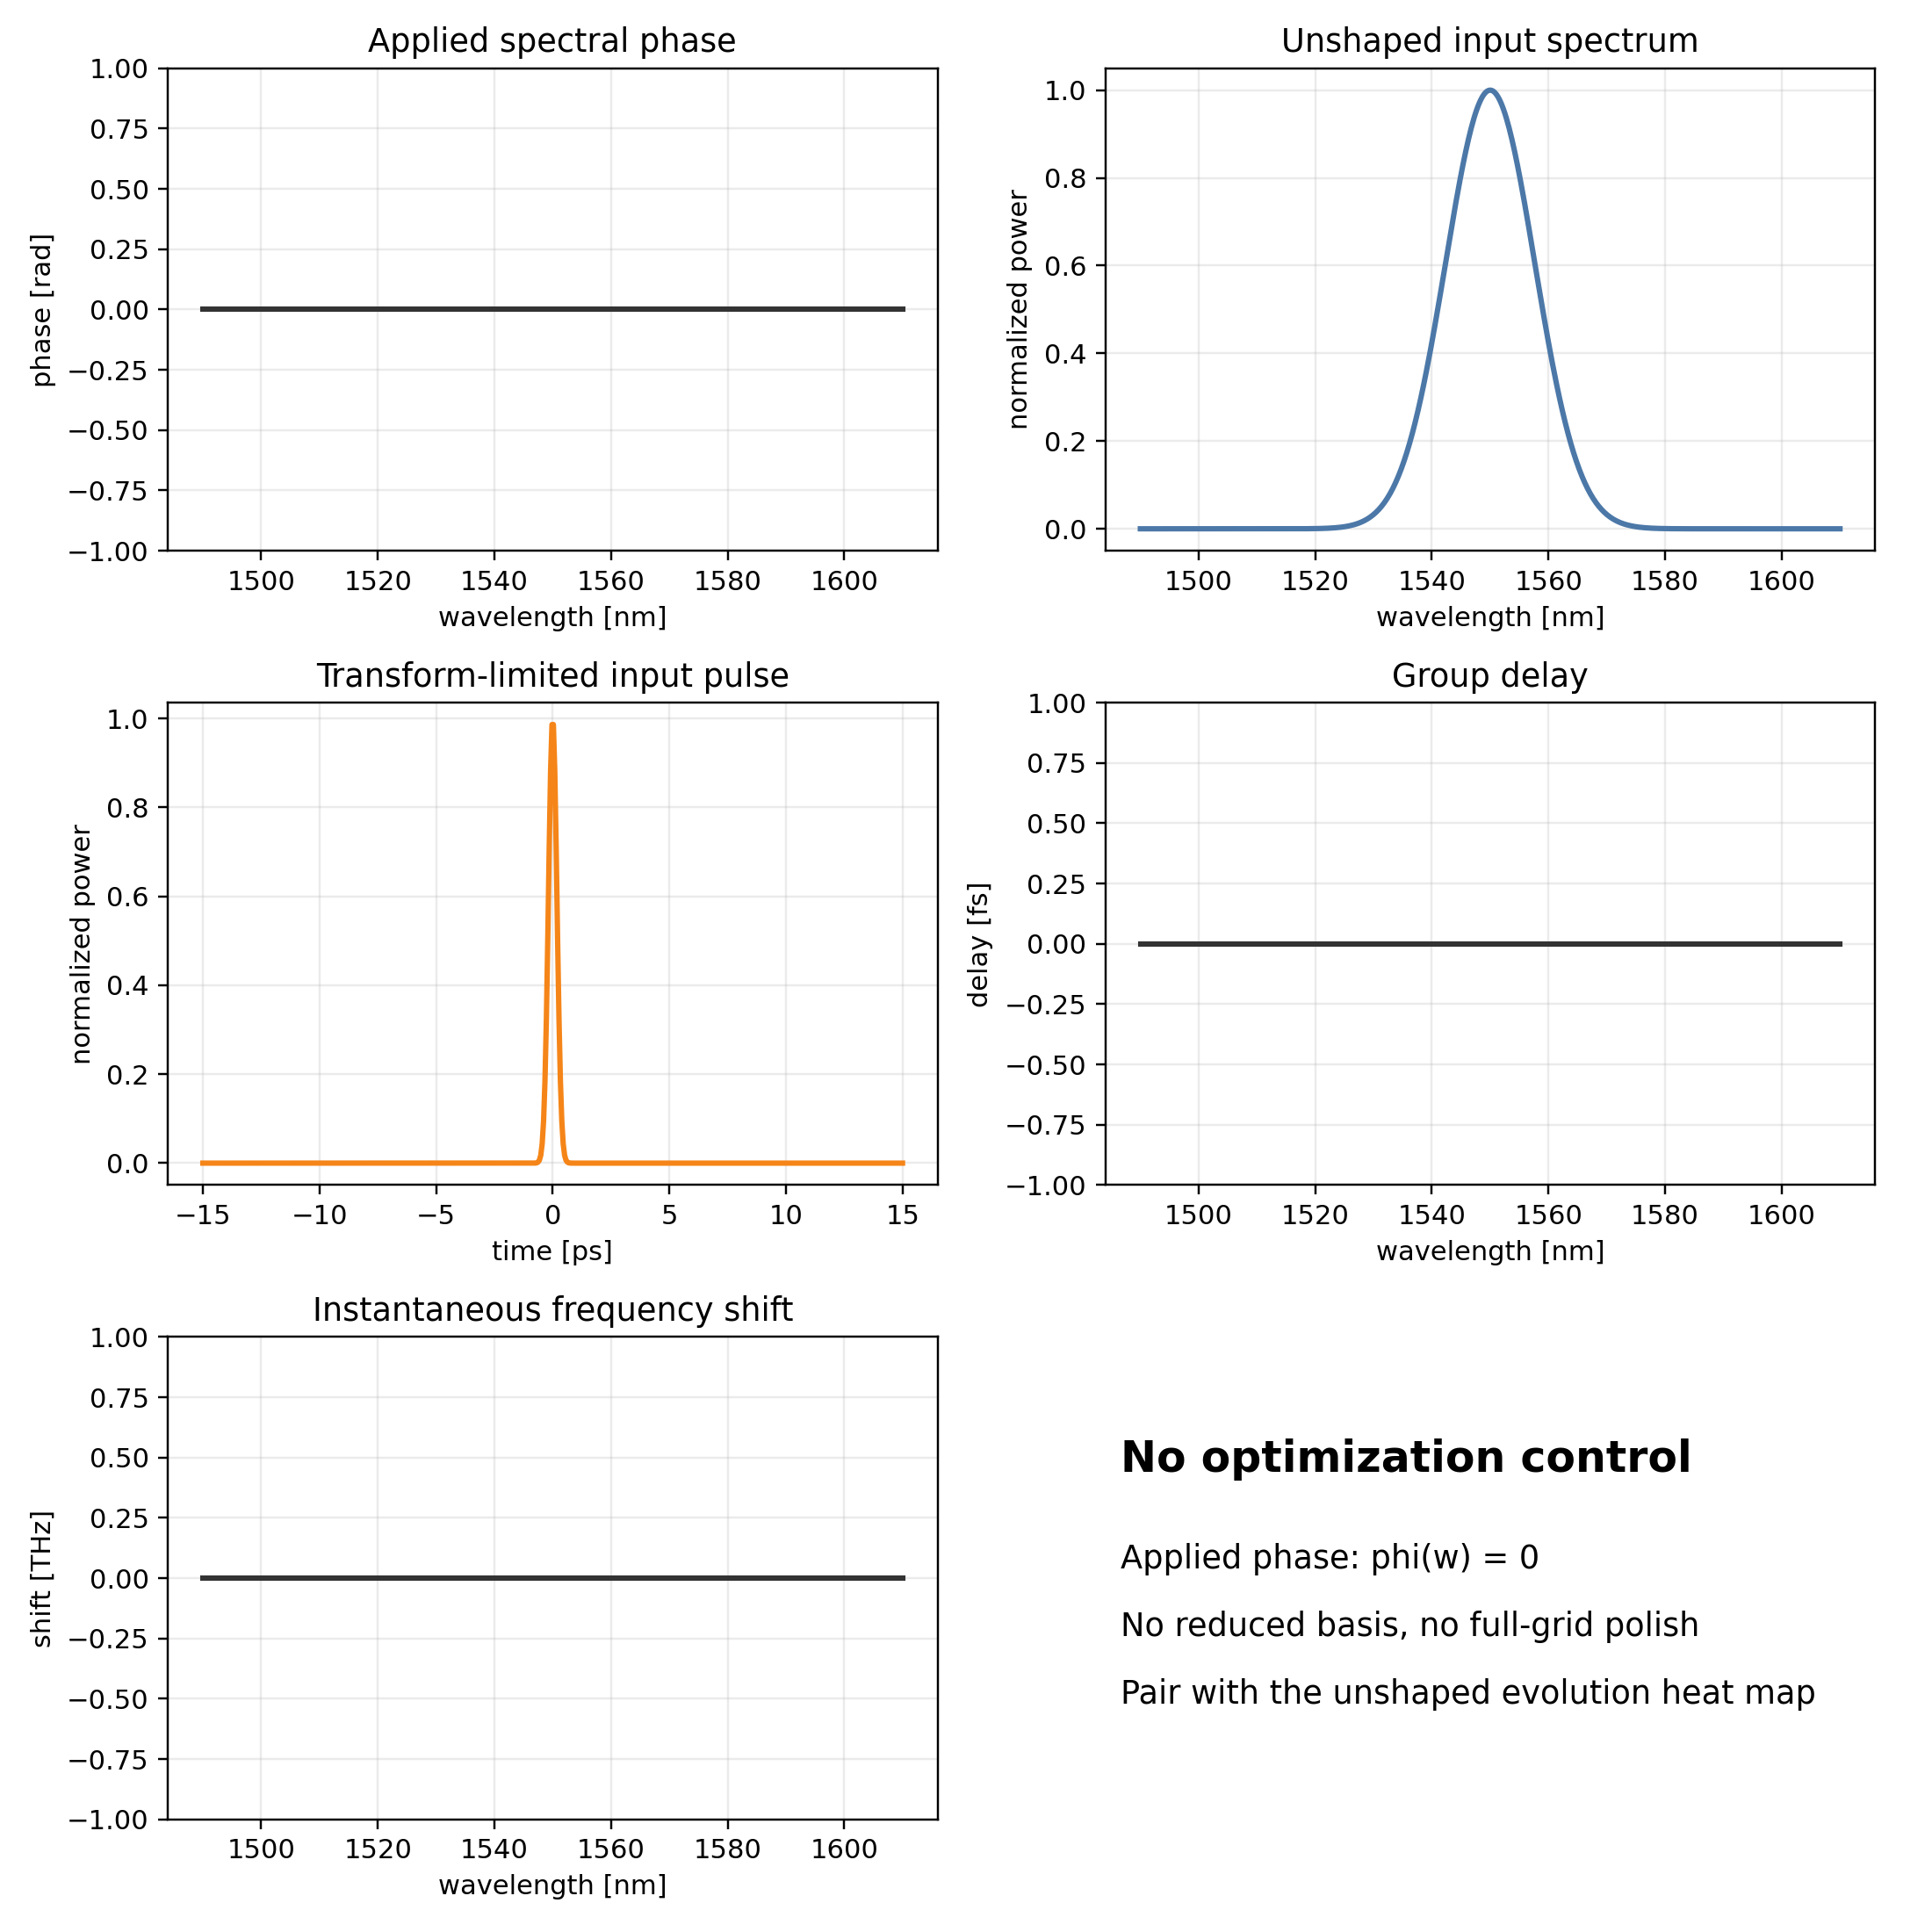
\includegraphics[height=0.47\textheight]{figures/no_optimization_phase_diagnostic.png}
\vspace{0.5em}

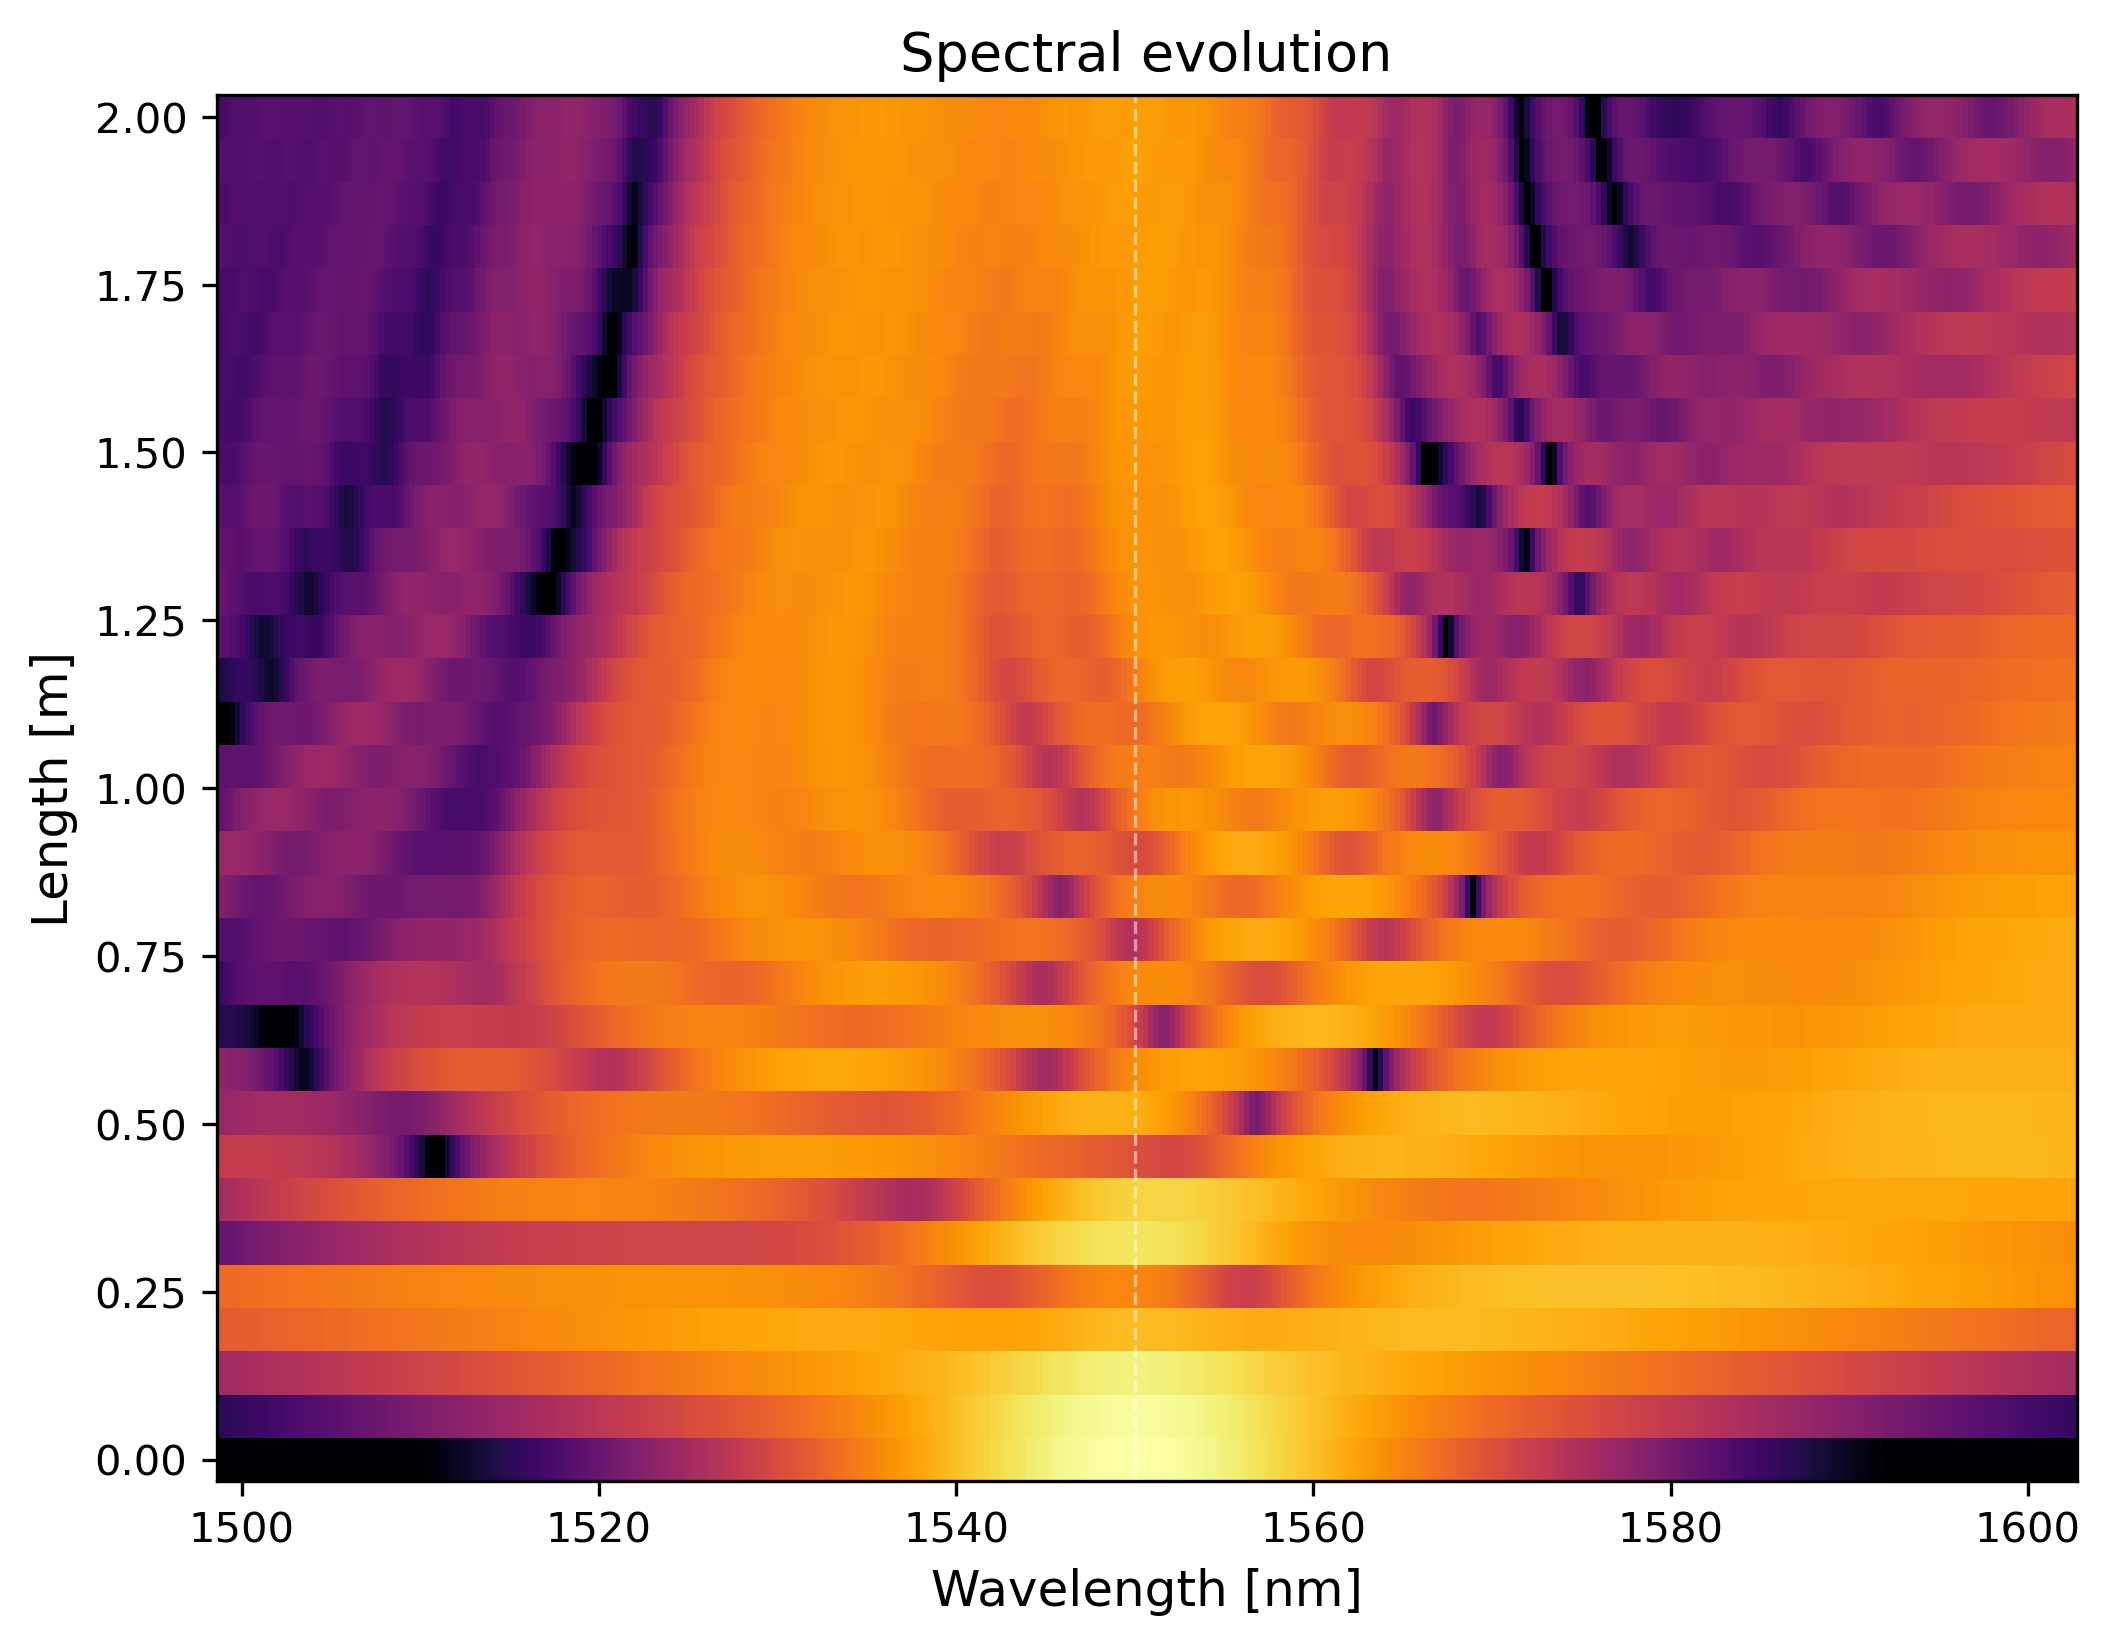
\includegraphics[height=0.31\textheight]{figures/canonical_smf28_evolution_unshaped.png}
\caption{No-optimization control for the canonical SMF-28 baseline. The phase
is flat, and the heat map shows the unshaped spectral evolution. This is the
reference page used to judge whether the optimized phase changed the dynamics.}
\end{figure}

\begin{figure}[p]
\centering
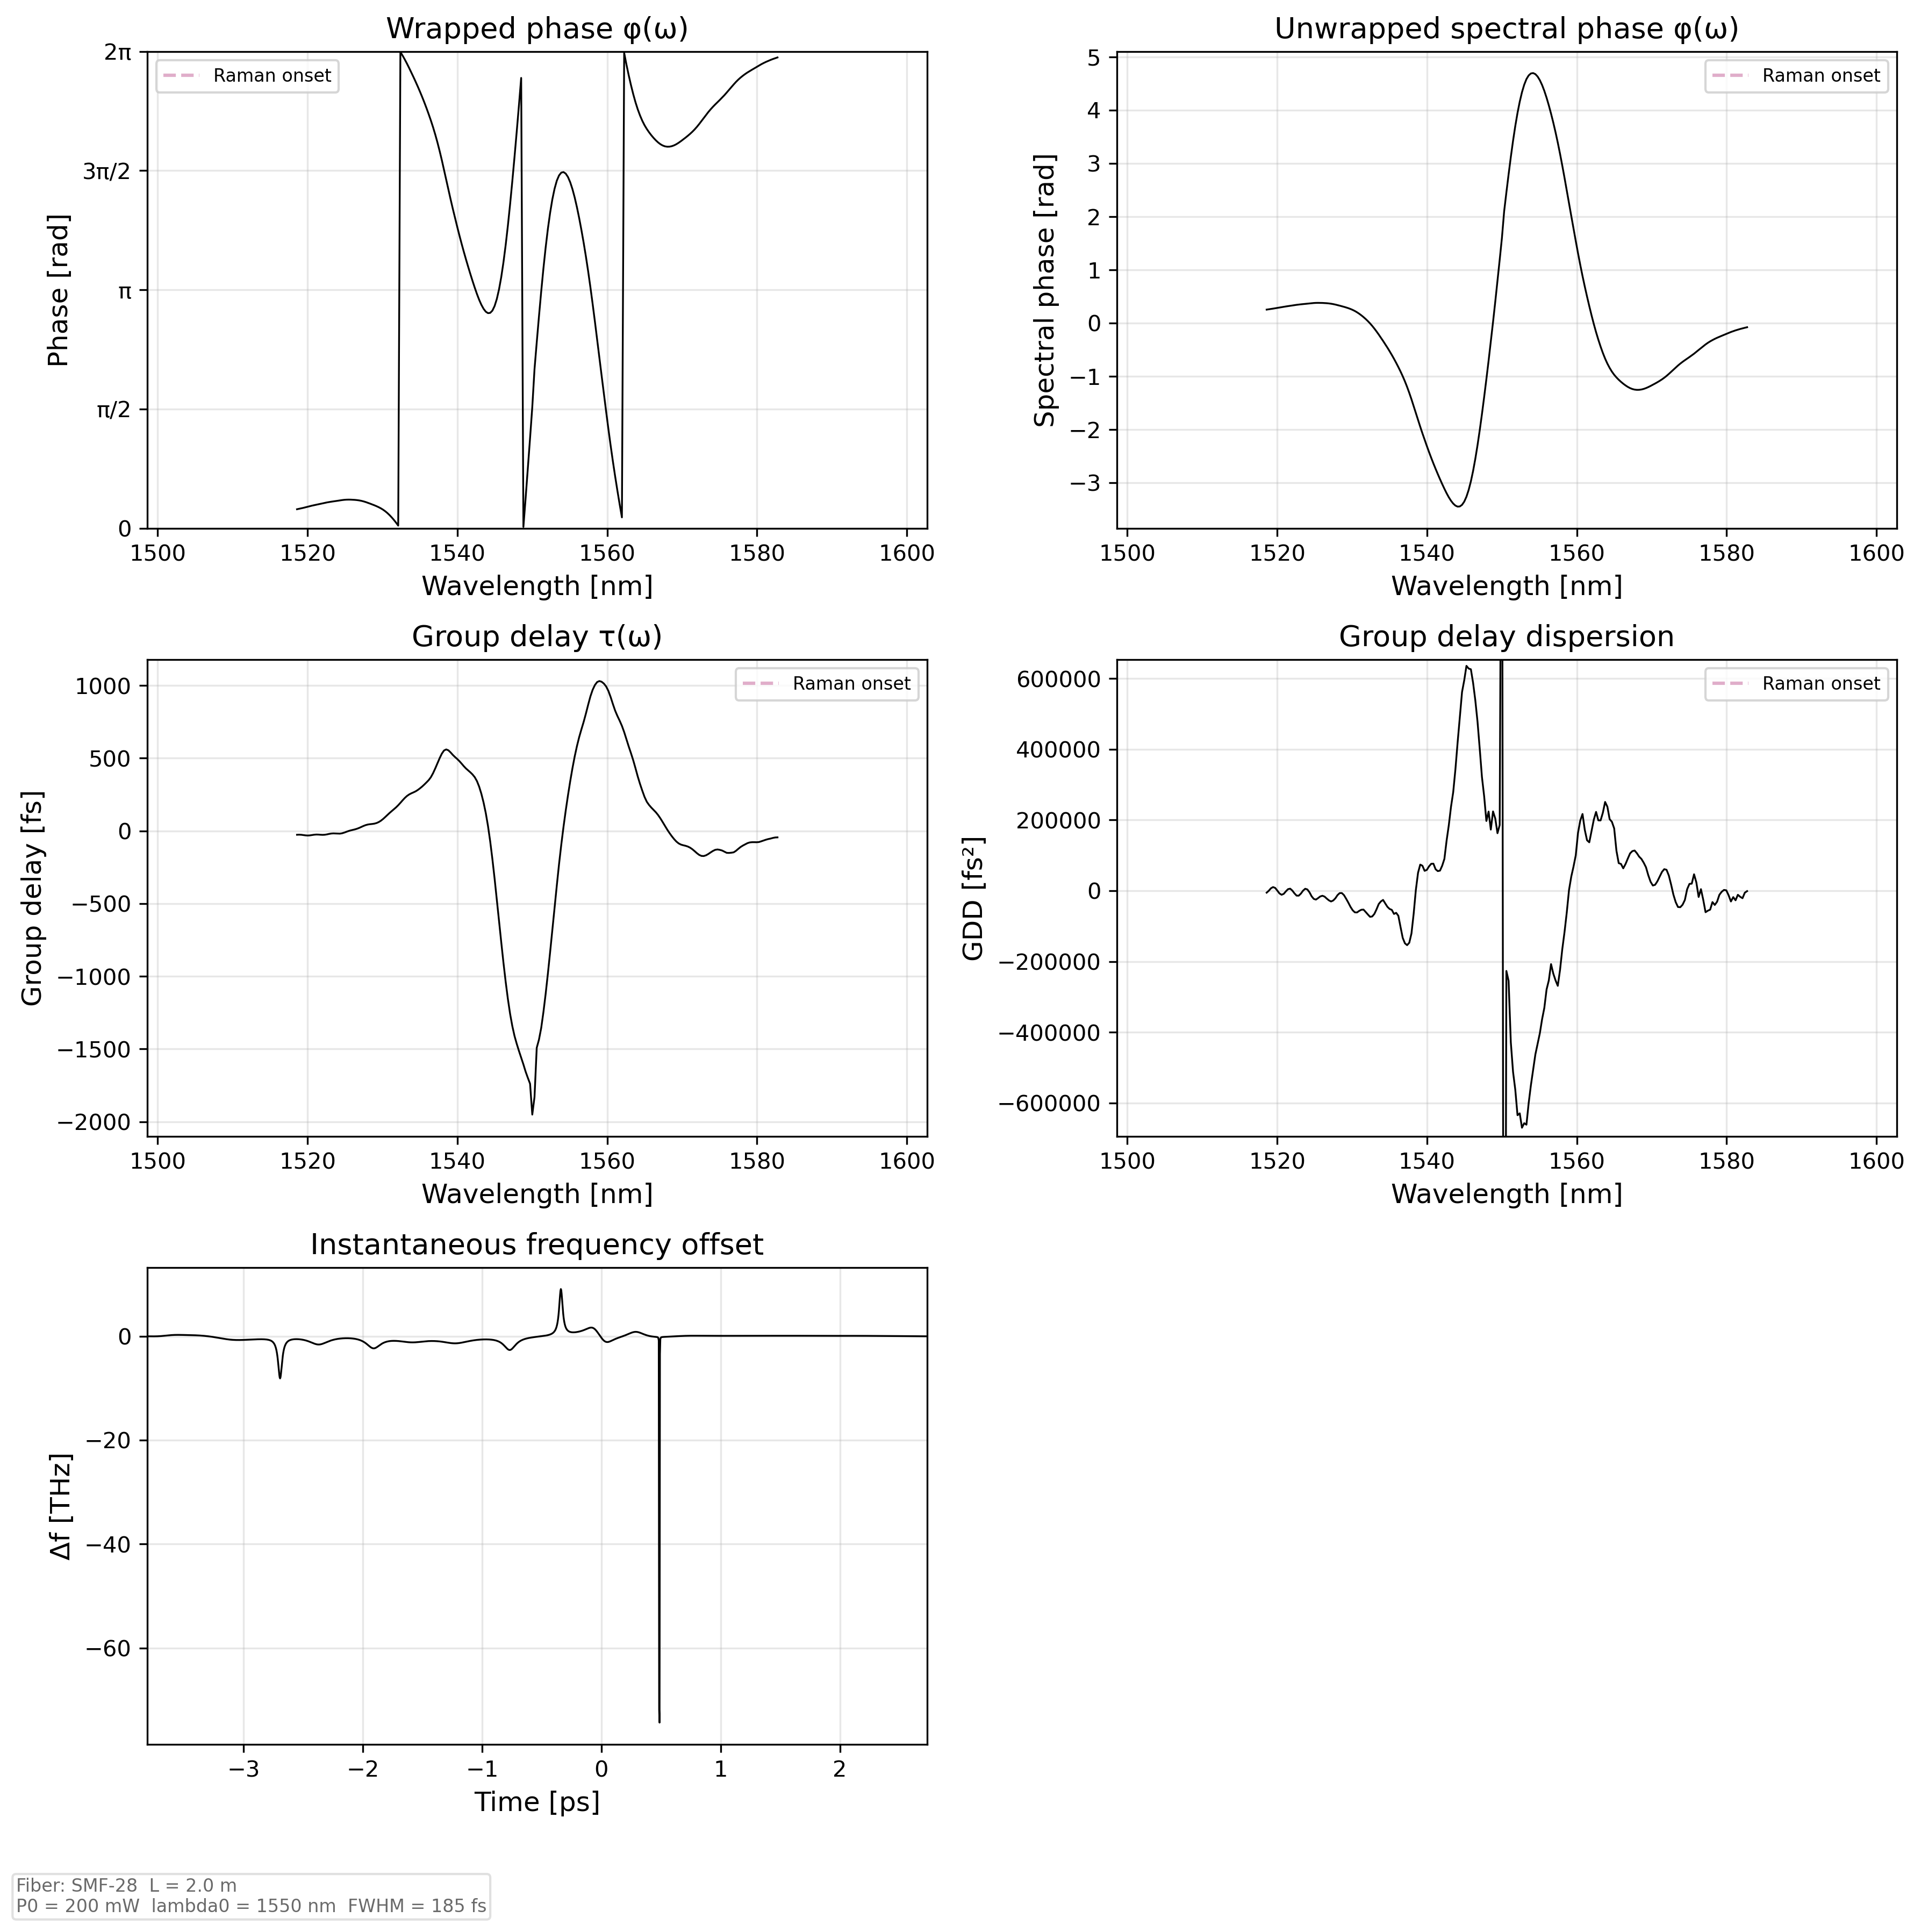
\includegraphics[height=0.47\textheight]{figures/canonical_smf28_phase_diagnostic.png}
\vspace{0.5em}

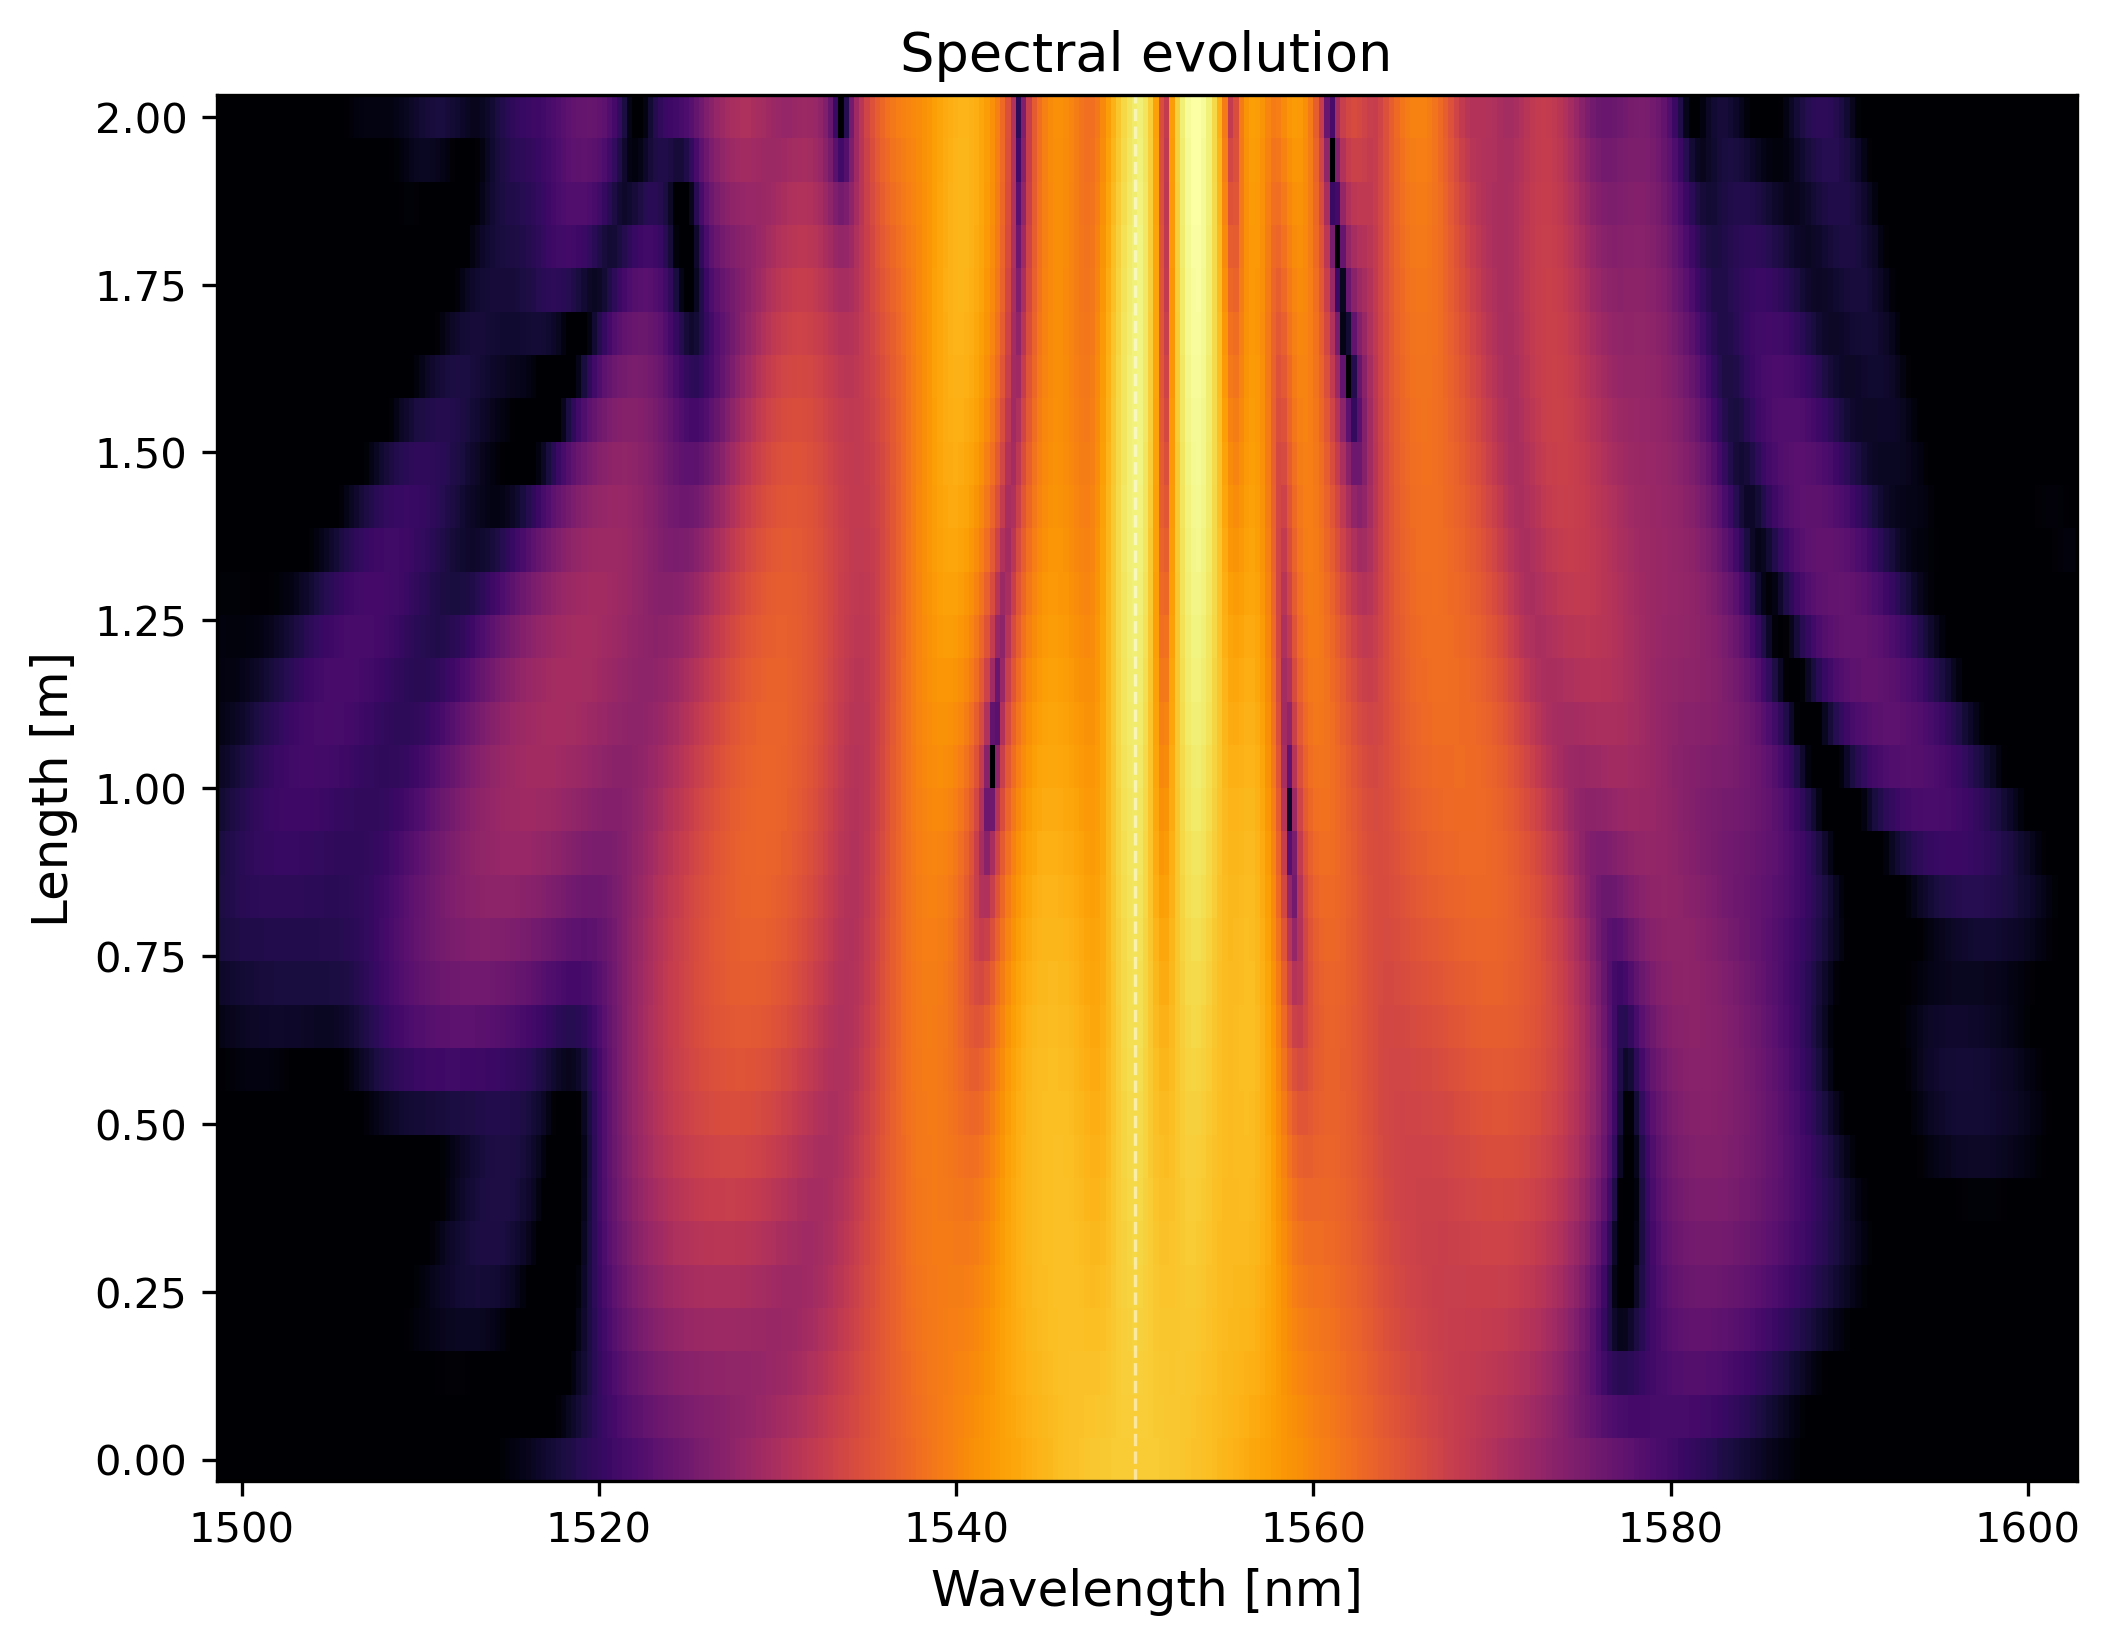
\includegraphics[height=0.31\textheight]{figures/canonical_smf28_evolution.png}
\caption{Optimized canonical SMF-28 baseline. The phase diagnostic shows the
mask produced by L-BFGS; the heat map shows the spectral evolution under that
mask. Read this page against the no-optimization control, not in isolation.}
\end{figure}

\begin{figure}[p]
\centering
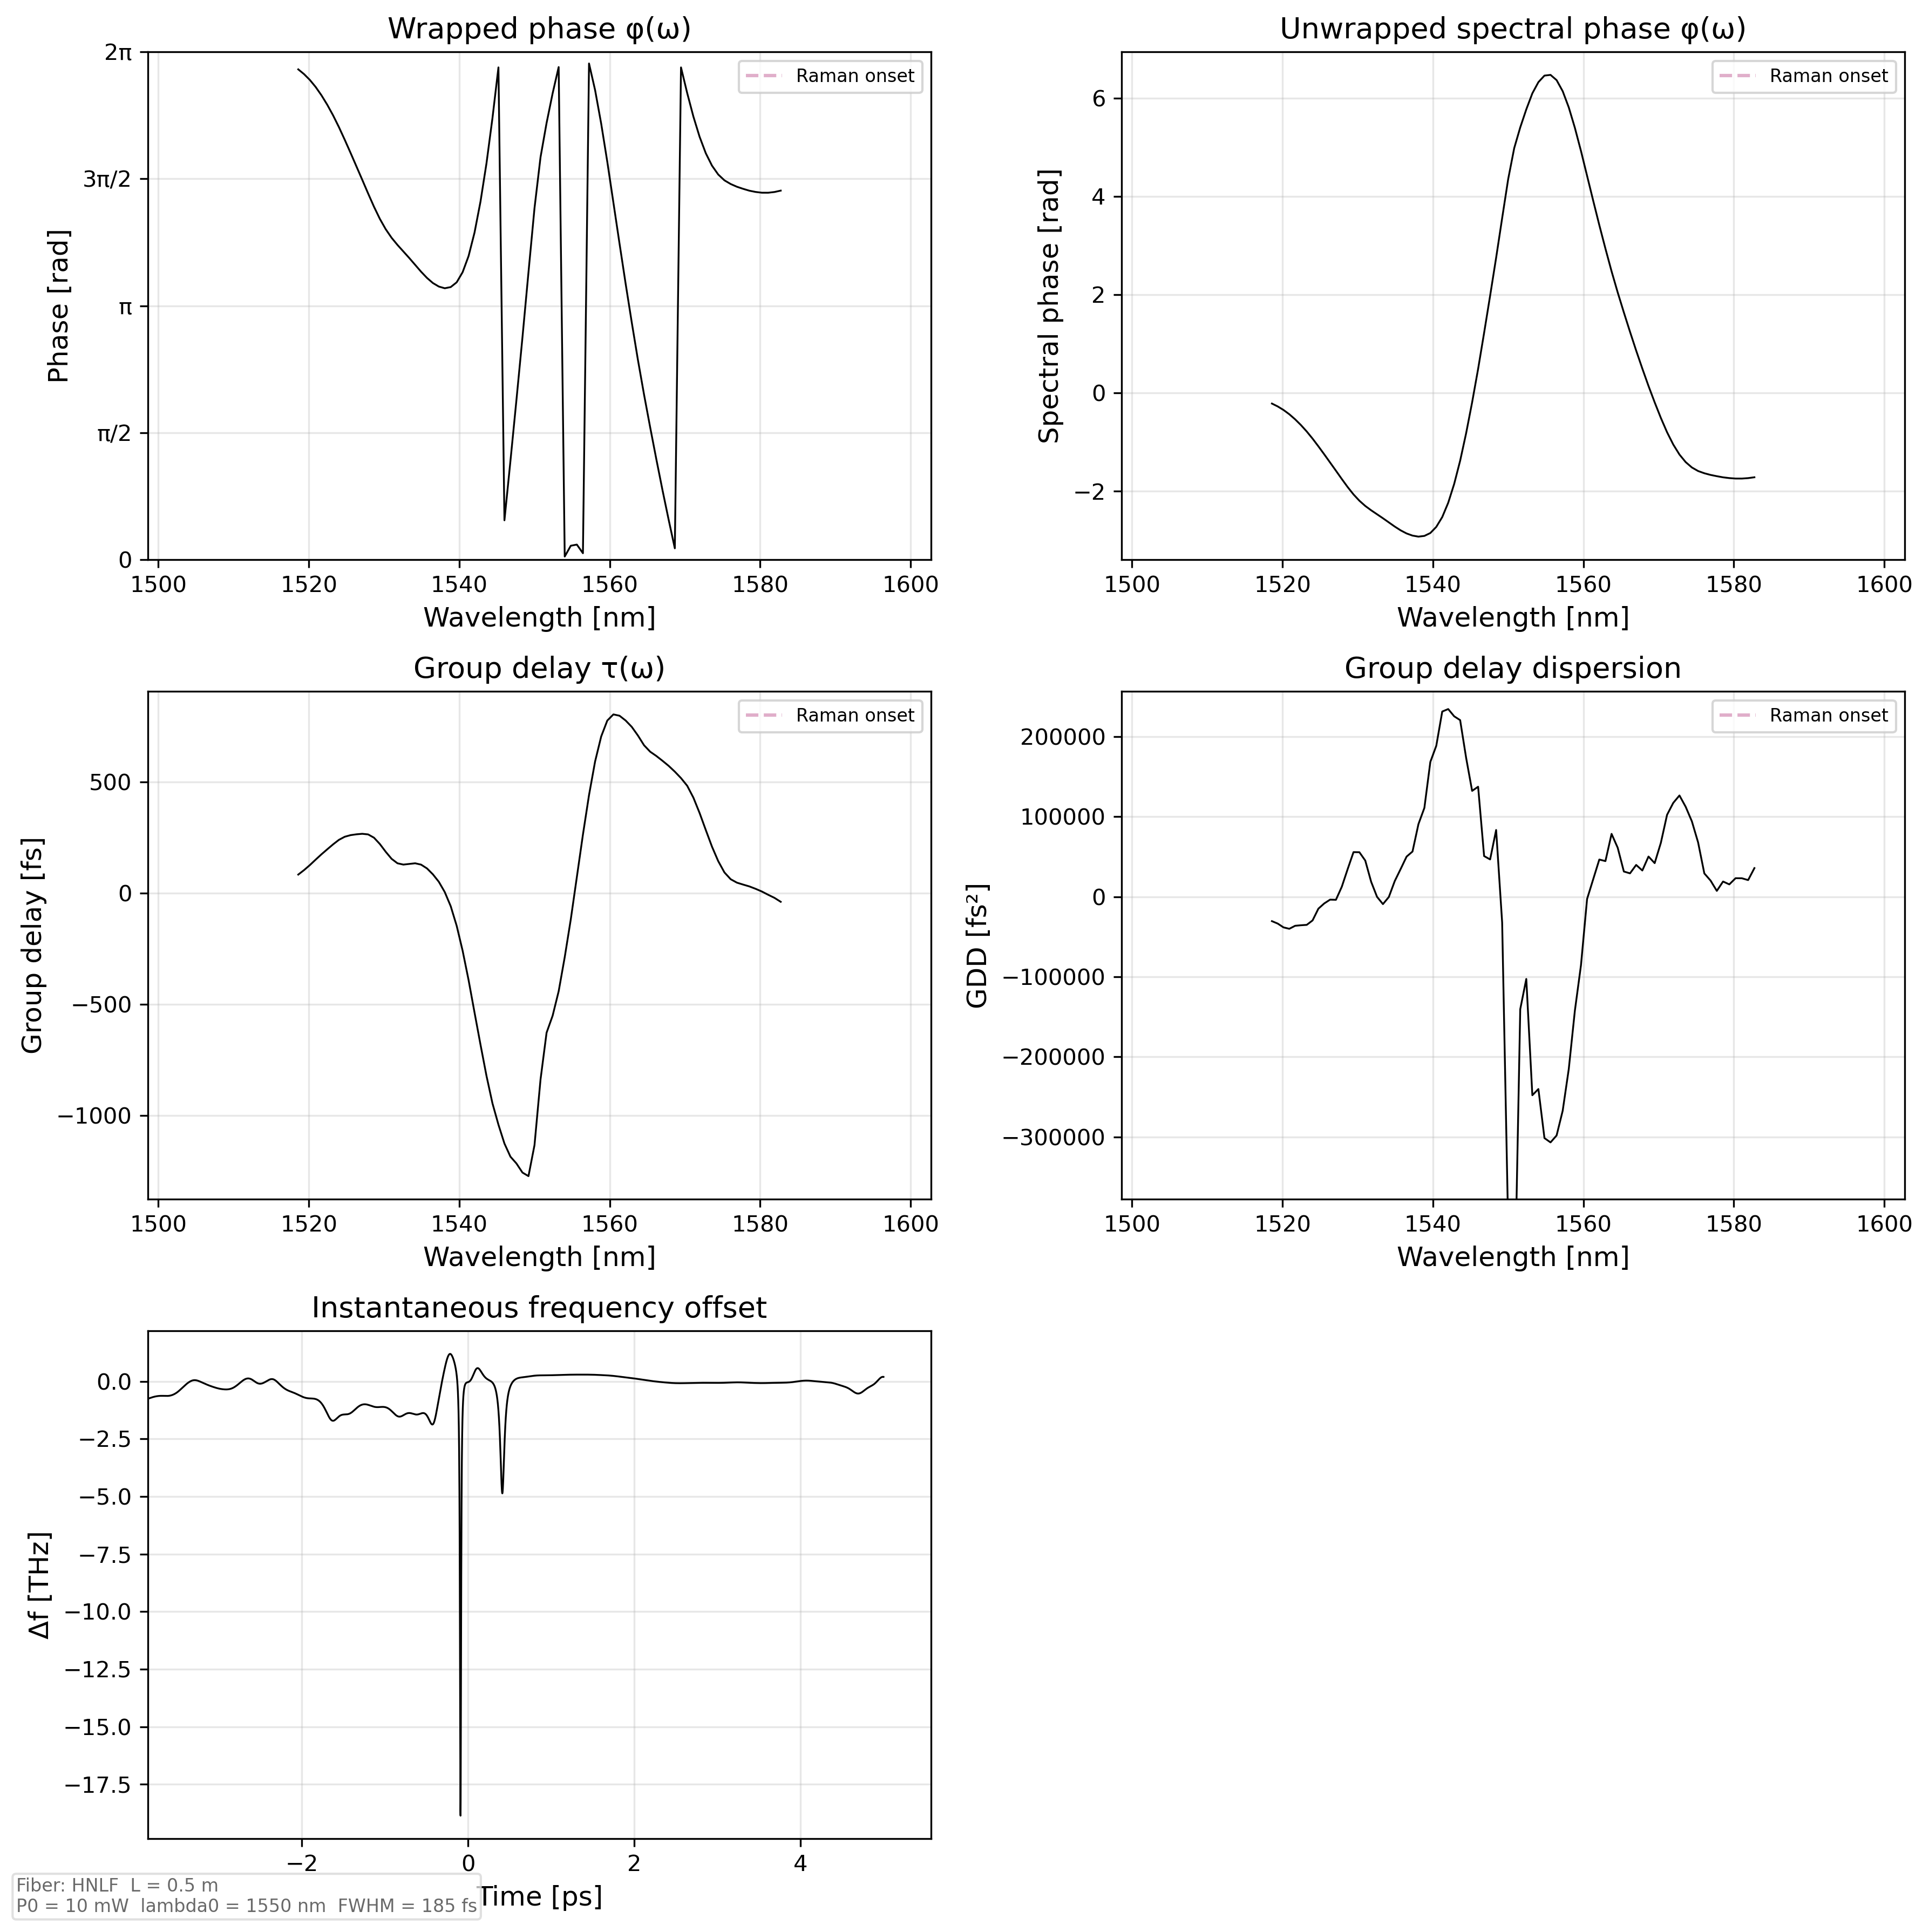
\includegraphics[height=0.47\textheight]{figures/reference_hnlf_phase_diagnostic.png}
\vspace{0.5em}

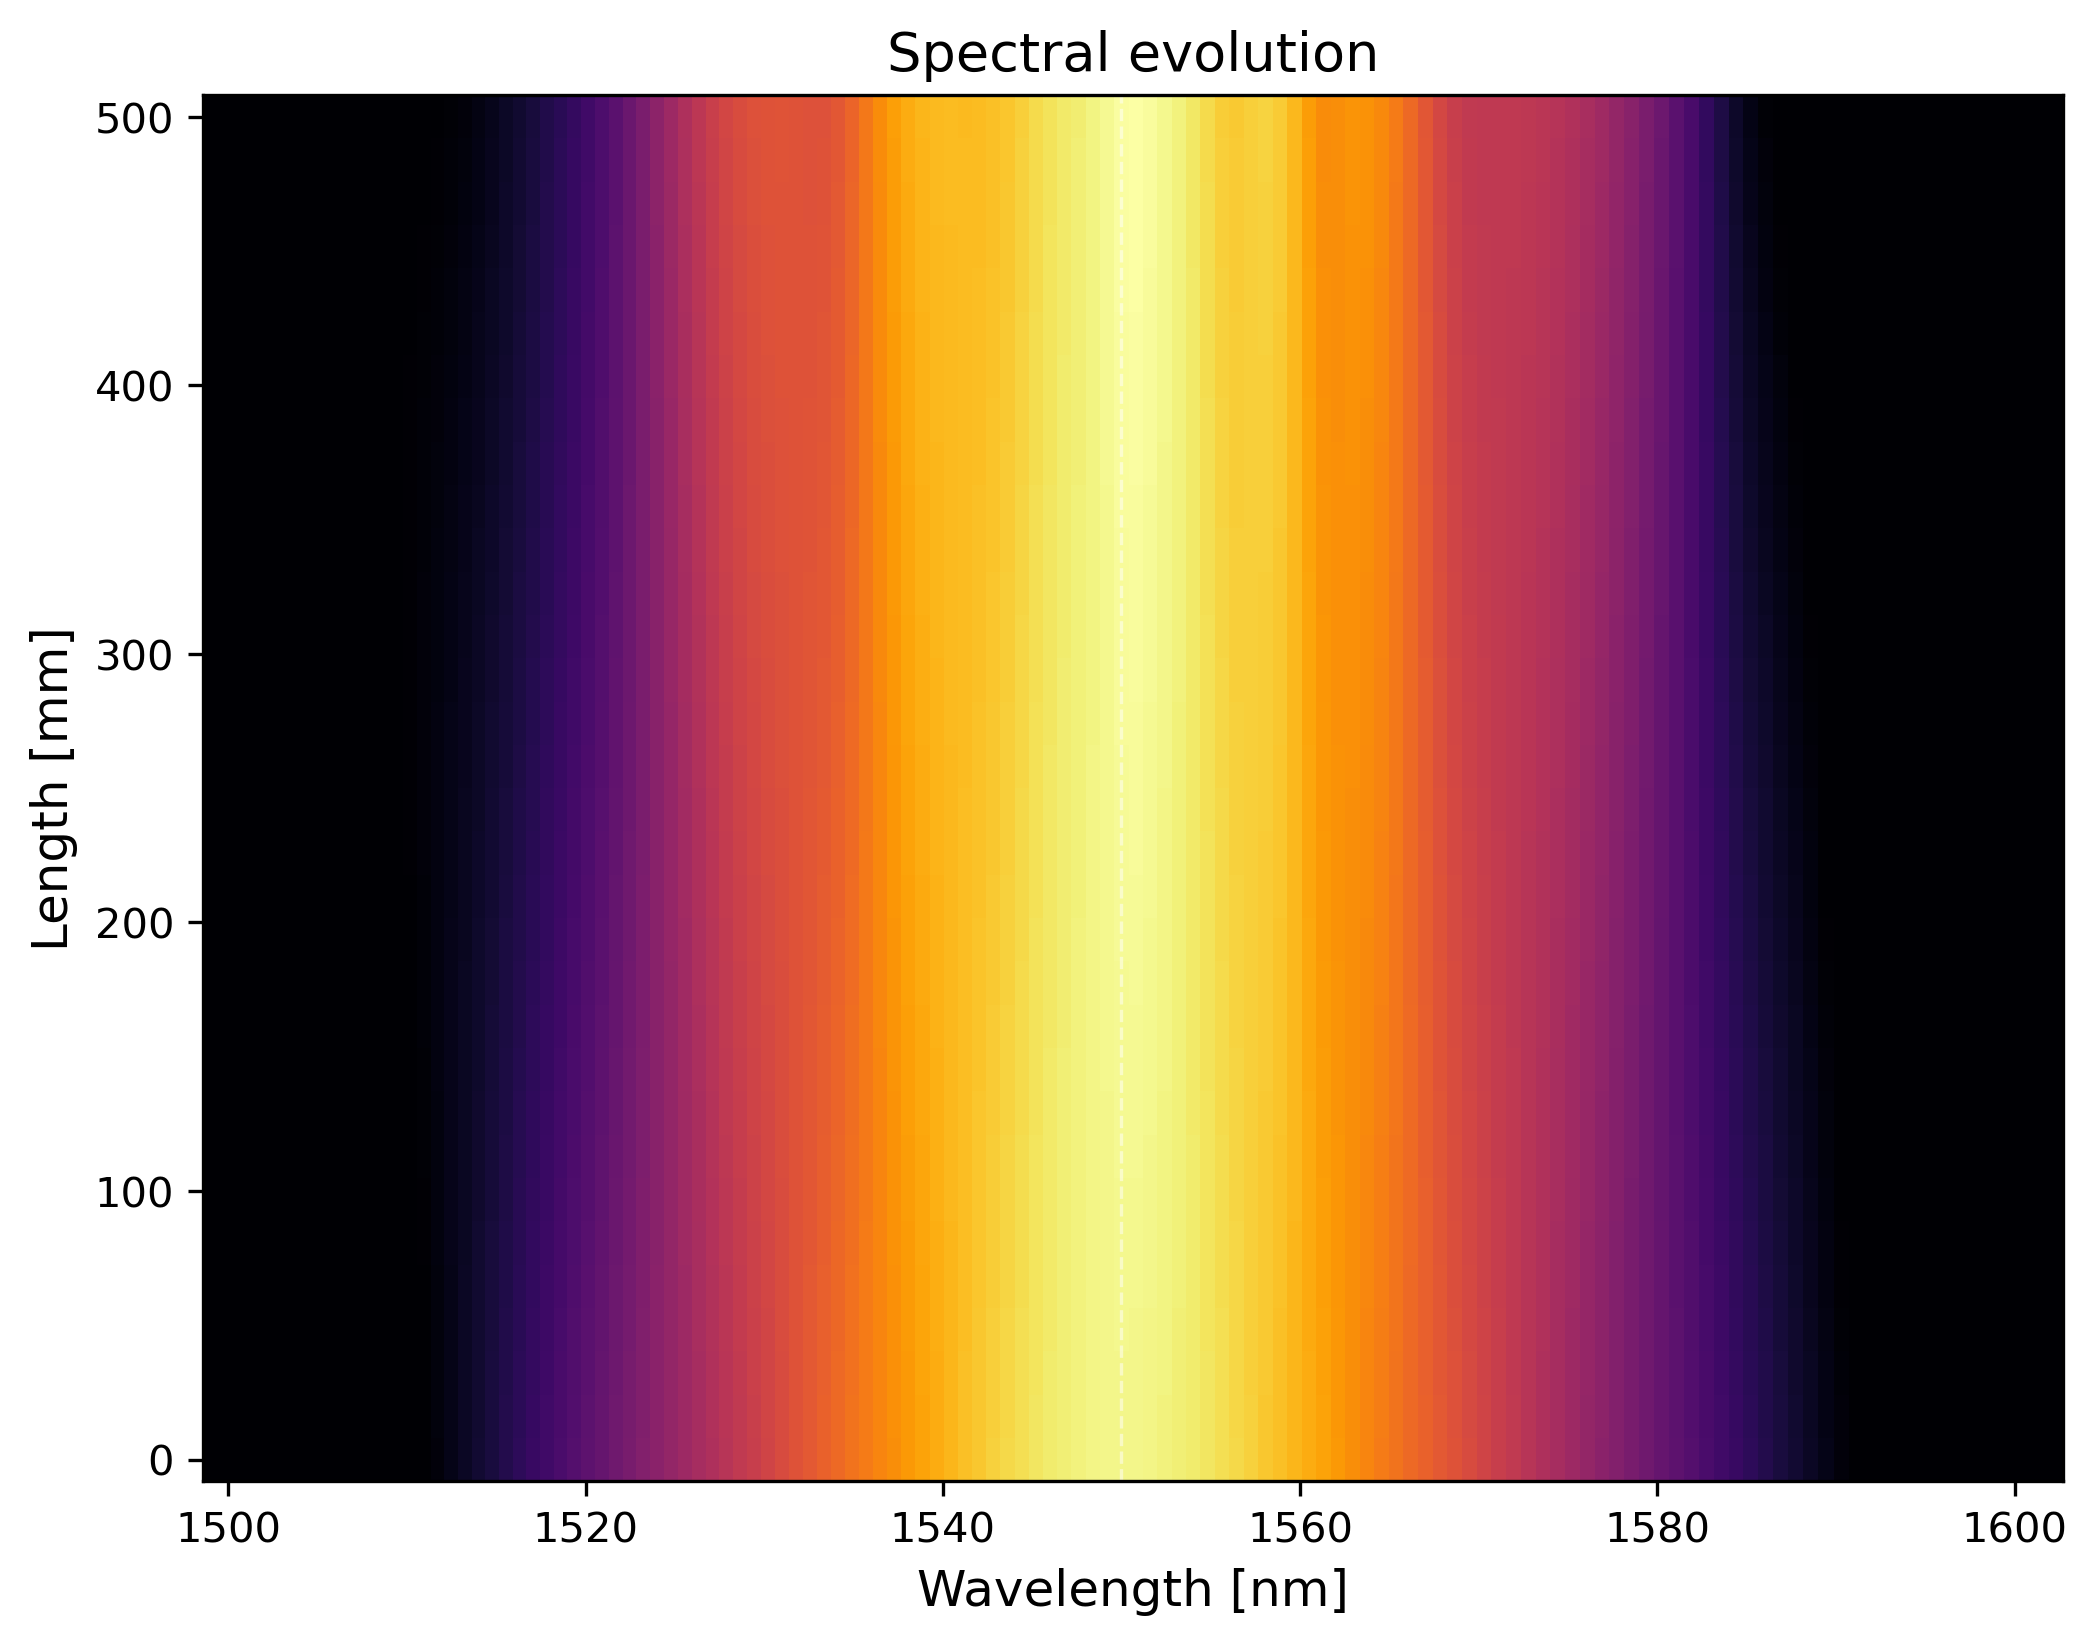
\includegraphics[height=0.31\textheight]{figures/reference_hnlf_evolution.png}
\caption{Reference single-mode HNLF run using the same phase-only diagnostic
language. This is not the canonical SMF-28 baseline, but it shows that the same
standard-image vocabulary transfers to another single-mode fiber setting.}
\end{figure}

\clearpage
\section{How To Read The Images}

\textbf{Wrapped phase.} This is \(\phi(\omega)\) modulo \(2\pi\). It is close
to what a phase modulator would implement.

\textbf{Unwrapped phase.} This removes \(2\pi\) jumps so the broad phase shape
is easier to see.

\textbf{Group delay.} This is the first derivative of phase with respect to
frequency. It describes which wavelengths are delayed or advanced.

\textbf{Group-delay dispersion.} This is the derivative of group delay. Large
spikes often indicate sharp phase structure and should be interpreted with
care.

\textbf{Spectral evolution heat map.} The x-axis is wavelength and the y-axis
is fiber length. Bright colors mean high spectral power. The important
question is how the shaped heat map differs from the unshaped control.

\subsection*{Intuition Check}

The phase diagnostic says what control was applied. The heat map says what the
fiber did in response. A convincing result should show both.

\section{Interpretation}

The baseline establishes that phase-only shaping can strongly change the
Raman-band output in the maintained single-mode setup. The canonical result is
not meant to be a universal best mask. It is meant to be the clean reference
case: one pulse, one fiber, one objective convention, one optimizer, one trust
report, and one standard image set.

This also explains why later notes are necessary. A mask that is deeper may be
less robust. A simpler mask may be easier to explain but shallower. A
second-order optimizer may find a different basin. Those are not contradictions
of the baseline; they are research directions built on top of it.

\section{Presentation Capsule}

If this note becomes the opening technical slide sequence, the clean message is:
\begin{itemize}
    \item The project optimizes an input spectral phase so less output energy lands in the Raman-shifted band.
    \item The baseline result is a clear no-shaping versus optimized comparison: \(-1.11\,\mathrm{dB}\) to \(-44.79\,\mathrm{dB}\) at the maintained SMF-28 point.
    \item The standard image set is part of the evidence: phase profile, phase diagnostic, optimized heat map, and no-shaping heat map.
    \item Later notes should be explained as modifications of this baseline: different parameterizations, objectives, optimizers, fibers, or validation rules.
\end{itemize}

\section{Limitations}

\textbf{Single-mode only.} This note does not establish multimode behavior.

\textbf{Phase-only only.} It does not compare against amplitude or joint
amplitude-phase shaping.

\textbf{Not a global optimum.} L-BFGS is local. The reported mask is a
trustworthy baseline result, not proof that no better phase exists.

\textbf{Objective-surface specific.} The canonical run uses the regularized dB
surface. Comparisons against physics-only linear costs, Hessian studies, or
different regularizers must name the surface explicitly.

\textbf{Images are necessary but not sufficient.} A human-facing PDF should
show the images, but the scalar metadata and trust checks still matter.

\section{Reproduction Capsule}

Canonical command:
\[
\texttt{julia -t auto --project=. scripts/canonical/optimize\_raman.jl}
\]
or, when available through the local workflow:
\[
\texttt{make optimize}
\]

Expected output is a timestamped directory under
\(\texttt{results/raman/smf28\_L2m\_P0p2W\_*}\) containing the result payload,
JSON sidecar, numerical trust report, and the standard image set:
\begin{itemize}
    \item phase profile image;
    \item phase diagnostic image;
    \item optimized spectral-evolution heat map;
    \item unshaped-control spectral-evolution heat map.
\end{itemize}

Substantial reruns should follow the project compute rules: use Julia with
threading enabled, run heavy simulations on the burst machine when appropriate,
and visually inspect the standard image set before calling the run complete.

\section{Sources and References}

\begin{thebibliography}{9}

\bibitem{agrawal2019}
G. P. Agrawal.
\textit{Nonlinear Fiber Optics}, 6th ed.
Academic Press, 2019.
\url{https://www.sciencedirect.com/book/9780128170427/nonlinear-fiber-optics}

\bibitem{dudley2006}
J. M. Dudley, G. Genty, and S. Coen.
``Supercontinuum generation in photonic crystal fiber.''
\textit{Reviews of Modern Physics}, 78, 1135--1184, 2006.
\url{https://doi.org/10.1103/RevModPhys.78.1135}

\bibitem{hult2007}
J. Hult.
``A fourth-order Runge-Kutta in the interaction picture method for simulating
supercontinuum generation in optical fibers.''
\textit{Journal of Lightwave Technology}, 25(12), 3770--3775, 2007.
\url{https://doi.org/10.1109/JLT.2007.909373}

\bibitem{gordon1986}
J. P. Gordon.
``Theory of the soliton self-frequency shift.''
\textit{Optics Letters}, 11(10), 662--664, 1986.
\url{https://doi.org/10.1364/OL.11.000662}

\bibitem{mitschke1986}
F. M. Mitschke and L. F. Mollenauer.
``Discovery of the soliton self-frequency shift.''
\textit{Optics Letters}, 11(10), 659--661, 1986.
\url{https://doi.org/10.1364/OL.11.000659}

\bibitem{liu1989}
D. C. Liu and J. Nocedal.
``On the limited memory BFGS method for large scale optimization.''
\textit{Mathematical Programming}, 45, 503--528, 1989.
\url{https://doi.org/10.1007/BF01589116}

\bibitem{nocedal2006}
J. Nocedal and S. J. Wright.
\textit{Numerical Optimization}, 2nd ed.
Springer, 2006.
\url{https://doi.org/10.1007/978-0-387-40065-5}

\end{thebibliography}

\end{document}
